\section{ATANH Inverse Hyperbolic Tangent Function}

\subsection{Usage}

Computes the inverse hyperbolic tangent of its argument.  The general
syntax for its use is
\begin{verbatim}
  y = atanh(x)
\end{verbatim}
where \verb|x| is an \verb|n|-dimensional array of numerical type.
\subsection{Function Internals}

The \verb|atanh| function is computed from the formula
\[
   \tanh^{-1}(x) = \frac{1}{2}\log\left(\frac{1+x}{1-x}\right)
\]
where the \verb|log| (and square root) is taken in its most general sense.
\subsection{Examples}

Here is a simple plot of the inverse hyperbolic tangent function
@>


\centerline{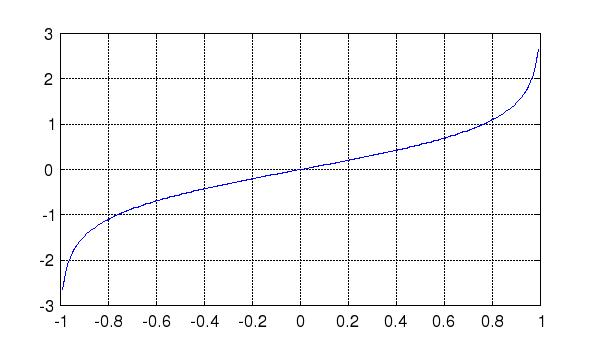
\includegraphics[width=8cm]{atanhplot}}

